\documentclass{standalone}

\usepackage{pgf}
\usepackage{tikz}
\usetikzlibrary{arrows,automata,matrix}
\usepackage[latin1]{inputenc}
\begin{document}
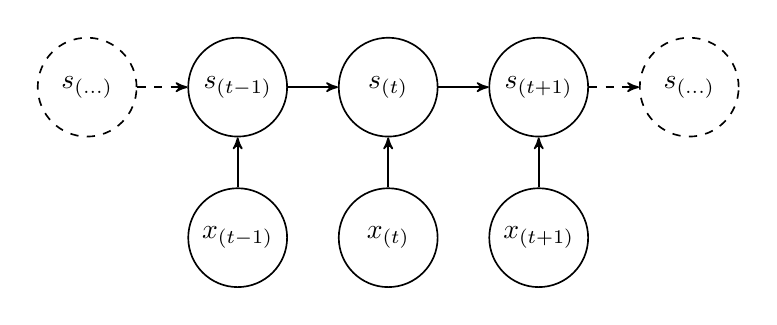
\begin{tikzpicture}[->,>=stealth'
	,shorten >=0pt
	,auto
	,node distance=2.8cm,
              semithick]
  \tikzstyle{every state}=[minimum size={10pt+width("$x_{(t-1)}$")}]

      \matrix (m) [matrix of nodes
      ,row sep=.25in,column sep=.25in]
      {
      %5 s's top row
      	\node[state,dashed](sd) {$s_{(\ldots)}$};	&
 	\node[state](stm1) {$s_{(t-1)}$};	 		&
 	\node[state](st) {$s_{(t)}$}; 					&
 	\node[state](stp1) {$s_{(t+1)}$};					&
 	\node[state,dashed](sd2) {$s_{(\ldots)}$}; 	\\
 	%3 xs btm
 											&
      \node[state](xtm1) {$x_{(t-1)}$}; 			&
      \node[state](xt) {$x_{(t)}$}; 				&
      \node[state](xtp1) {$x_{(t+1)}$} ;			\\
      };
    
  \path[dashed]  (sd) edge       node {} (stm1);
  \path 
 	(xtm1) edge  node {} (stm1)
 	(stm1) edge       node {} (st)
 	(xt) edge  node {} (st)
 	(st) edge       node {} (stp1)
 	(xtp1) edge  node {} (stp1);
 \path[dashed] (stp1) edge       node {} (sd2)
 	;
 
\end{tikzpicture}

\end{document}